% ******************************* PhD Thesis Template **************************
% Please have a look at the README.md file for info on how to use the template

\documentclass[a4paper,12pt,times,numbered,print,index]{Classes/PhDThesisPSnPDF}

% ******************************************************************************
% ******************************* Class Options ********************************
% *********************** See README for more details **************************
% ******************************************************************************

% `a4paper'(The University of Cambridge PhD thesis guidelines recommends a page
% size a4 - default option) or `a5paper': A5 Paper size is also allowed as per
% the Cambridge University Engineering Deparment guidelines for PhD thesis
%
% `11pt' or `12pt'(default): Font Size 10pt is NOT recommended by the University
% guidelines
%
% `oneside' or `twoside'(default): Printing double side (twoside) or single
% side.
%
% `print': Use `print' for print version with appropriate margins and page
% layout. Leaving the options field blank will activate Online version.
%
% `index': For index at the end of the thesis
%
% `draftclassic': For draft mode without loading any images (same as draft in book)
%
% `draft': Special draft mode with line numbers, images, and water mark with
% timestamp and custom text. Position of the text can also be modified.
%
% `abstract': To generate only the title page and abstract page with
% dissertation title and name, to submit to the Student Registry
%
% `chapter`: This option enables only the specified chapter and it's references
%  Useful for review and corrections.
%
% ************************* Custom Page Margins ********************************
%
% `custommargin`: Use `custommargin' in options to activate custom page margins,
% which can be defined in the preamble.tex. Custom margin will override
% print/online margin setup.
%
% *********************** Choosing the Fonts in Class Options ******************
%
% `times' : Times font with math support. (The Cambridge University guidelines
% recommend using times)
%
% `fourier': Utopia Font with Fourier Math font (Font has to be installed)
%            It's a free font.
%
% `customfont': Use `customfont' option in the document class and load the
% package in the preamble.tex
%
% default or leave empty: `Latin Modern' font will be loaded.
%
% ********************** Choosing the Bibliography style ***********************
%
% `authoryear': For author-year citation eg., Krishna (2013)
%
% `numbered': (Default Option) For numbered and sorted citation e.g., [1,5,2]
%
% `custombib': Define your own bibliography style in the `preamble.tex' file.
%              `\RequirePackage[square, sort, numbers, authoryear]{natbib}'.
%              This can be also used to load biblatex instead of natbib
%              (See Preamble)
%
% **************************** Choosing the Page Style *************************
%
% `default (leave empty)': For Page Numbers in Header (Left Even, Right Odd) and
% Chapter Name in Header (Right Even) and Section Name (Left Odd). Blank Footer.
%
% `PageStyleI': Chapter Name next & Page Number on Even Side (Left Even).
% Section Name & Page Number in Header on Odd Side (Right Odd). Footer is empty.
%
% `PageStyleII': Chapter Name on Even Side (Left Even) in Header. Section Number
% and Section Name in Header on Odd Side (Right Odd). Page numbering in footer


% ********************************** Preamble **********************************
% Preamble: Contains packages and user-defined commands and settings
% ******************************************************************************
% ****************************** Custom Margin *********************************

% Add `custommargin' in the document class options to use this section
% Set {innerside margin / outerside margin / topmargin / bottom margin}  and
% other page dimensions
\ifsetCustomMargin
  \RequirePackage[left=37mm,right=30mm,top=35mm,bottom=30mm]{geometry}
  \setFancyHdr % To apply fancy header after geometry package is loaded
\fi

% Add spaces between paragraphs
%\setlength{\parskip}{0.5em}
% Ragged bottom avoids extra whitespaces between paragraphs
\raggedbottom
% To remove the excess top spacing for enumeration, list and description
%\usepackage{enumitem}
%\setlist[enumerate,itemize,description]{topsep=0em}

% *****************************************************************************
% ******************* Fonts (like different typewriter fonts etc.)*************

% Add `customfont' in the document class option to use this section

\ifsetCustomFont
  % Set your custom font here and use `customfont' in options. Leave empty to
  % load computer modern font (default LaTeX font).
  %\RequirePackage{helvet}

  % For use with XeLaTeX
  %  \setmainfont[
  %    Path              = ./libertine/opentype/,
  %    Extension         = .otf,
  %    UprightFont = LinLibertine_R,
  %    BoldFont = LinLibertine_RZ, % Linux Libertine O Regular Semibold
  %    ItalicFont = LinLibertine_RI,
  %    BoldItalicFont = LinLibertine_RZI, % Linux Libertine O Regular Semibold Italic
  %  ]
  %  {libertine}
  %  % load font from system font
  %  \newfontfamily\libertinesystemfont{Linux Libertine O}
\fi

% *****************************************************************************
% **************************** Custom Packages ********************************

% ************************* Algorithms and Pseudocode **************************

%\usepackage{algpseudocode}


% ********************Captions and Hyperreferencing / URL **********************

% Captions: This makes captions of figures use a boldfaced small font.
%\RequirePackage[small,bf]{caption}

\RequirePackage[labelsep=space,tableposition=top]{caption}
\renewcommand{\figurename}{Fig.} %to support older versions of captions.sty


% *************************** Graphics and figures *****************************

%\usepackage{rotating}
%\usepackage{wrapfig}

% Uncomment the following two lines to force Latex to place the figure.
% Use [H] when including graphics. Note 'H' instead of 'h'
%\usepackage{float}
%\restylefloat{figure}

% Subcaption package is also available in the sty folder you can use that by
% uncommenting the following line
% This is for people stuck with older versions of texlive
%\usepackage{sty/caption/subcaption}
\usepackage{subcaption}

% ********************************** Tables ************************************
\usepackage{booktabs} % For professional looking tables
\usepackage{./sty/multirow}

%\usepackage{multicol}
%\usepackage{longtable}
%\usepackage{tabularx}


% *********************************** SI Units *********************************
\usepackage{./sty/siunitx} % use this package module for SI units


% ******************************* Line Spacing *********************************

% Choose linespacing as appropriate. Default is one-half line spacing as per the
% University guidelines

% \doublespacing
% \onehalfspacing
% \singlespacing


% ************************ Formatting / Footnote *******************************

% Don't break enumeration (etc.) across pages in an ugly manner (default 10000)
%\clubpenalty=500
%\widowpenalty=500

%\usepackage[perpage]{footmisc} %Range of footnote options


% *****************************************************************************
% *************************** Bibliography  and References ********************

%\usepackage{cleveref} %Referencing without need to explicitly state fig /table

% Add `custombib' in the document class option to use this section
\ifuseCustomBib
   \RequirePackage[square, sort, numbers, authoryear]{natbib} % CustomBib

% If you would like to use biblatex for your reference management, as opposed to the default `natbibpackage` pass the option `custombib` in the document class. Comment out the previous line to make sure you don't load the natbib package. Uncomment the following lines and specify the location of references.bib file

%\RequirePackage[backend=biber, style=numeric-comp, citestyle=numeric, sorting=nty, natbib=true]{biblatex}
%\bibliography{References/references} %Location of references.bib only for biblatex

\fi

% changes the default name `Bibliography` -> `References'
\renewcommand{\bibname}{References}


% ******************************************************************************
% ************************* User Defined Commands ******************************
% ******************************************************************************

% *********** To change the name of Table of Contents / LOF and LOT ************

%\renewcommand{\contentsname}{My Table of Contents}
%\renewcommand{\listfigurename}{My List of Figures}
%\renewcommand{\listtablename}{My List of Tables}


% ********************** TOC depth and numbering depth *************************

\setcounter{secnumdepth}{2}
\setcounter{tocdepth}{2}


% ******************************* Nomenclature *********************************

% To change the name of the Nomenclature section, uncomment the following line

%\renewcommand{\nomname}{Symbols}


% ********************************* Appendix ***********************************

% The default value of both \appendixtocname and \appendixpagename is `Appendices'. These names can all be changed via:

%\renewcommand{\appendixtocname}{List of appendices}
%\renewcommand{\appendixname}{Appndx}

% *********************** Configure Draft Mode **********************************

% Uncomment to disable figures in `draft'
%\setkeys{Gin}{draft=true}  % set draft to false to enable figures in `draft'

% These options are active only during the draft mode
% Default text is "Draft"
%\SetDraftText{DRAFT}

% Default Watermark location is top. Location (top/bottom)
%\SetDraftWMPosition{bottom}

% Draft Version - default is v1.0
%\SetDraftVersion{v1.1}

% Draft Text grayscale value (should be between 0-black and 1-white)
% Default value is 0.75
%\SetDraftGrayScale{0.8}


% ******************************** Todo Notes **********************************
%% Uncomment the following lines to have todonotes.

%\ifsetDraft
%	\usepackage[colorinlistoftodos]{todonotes}
%	\newcommand{\mynote}[1]{\todo[author=kks32,size=\small,inline,color=green!40]{#1}}
%\else
%	\newcommand{\mynote}[1]{}
%	\newcommand{\listoftodos}{}
%\fi

% Example todo: \mynote{Hey! I have a note}


% ************************ Thesis Information & Meta-data **********************
% Thesis title and author information, refernce file for biblatex
% ************************ Thesis Information & Meta-data **********************
%% The title of the thesis
\title{Functional methods in agent-based computational economics}
%\texorpdfstring is used for PDF metadata. Usage:
%\texorpdfstring{LaTeX_Version}{PDF Version (non-latex)} eg.,
%\texorpdfstring{$sigma$}{sigma}

%% Subtitle (Optional)
\subtitle{Novel approaches for implementing ACE models}

%% The full name of the author
\author{Jonathan Andreas Thaler}

%% Department (eg. Department of Engineering, Maths, Physics)
\dept{Department of Computer Science}

%% University and Crest
\university{University of Nottingham}
% Crest minimum should be 30mm.
\crest{
\includegraphics[width=0.7\textwidth]{University_Nottingham_LOGO}}
%% Use this crest, if you are using the college crest
%% Crest long miminum should be 65mm
%\crest{
\includegraphics[width=0.45\textwidth]{University_Crest_Long}}

%% College shield [optional] 
% Crest minimum should be 30mm.
%\collegeshield{
\includegraphics[width=0.2\textwidth]{CollegeShields/Kings}}


%% Supervisor (optional)
%% for multiple supervisors, append each supervisor with the \newline command
\supervisor{\textbf{Prof. Peer-Olaf Siebers \newline
Prof. Thorsten Altenkirch}}

%% Supervisor Role (optional) - Supervisor (default) or advisor
% \supervisorrole{\textbf{Supervisors: }}
%% if no title is desired:
% \supervisorrole{}

%% Advisor (optional)
%% for multiple advisors, append each advisor with the \newline command
%\advisor{Advisor 1\newline
%Advisors 2\newline
%Advisor 3\newline
%Advisor 4}
     
%% Advisor Role (optional) - Advisor (default) or leave empty
% \advisorrole{Advisors: }
%% if no title is required
% \advisorrole{}


%% You can redefine the submission text:
% Default as per the University guidelines:
% ``This dissertation is submitted for the degree of''
%\renewcommand{\submissiontext}{change the default text here if needed}

%% Full title of the Degree
\degreetitle{Doctor of Philosophy}

%% College affiliation (optional)
% \college{King's College}

%% Submission date
% Default is set as {\monthname[\the\month]\space\the\year}
%\degreedate{September 2014} 

%% Meta information
\subject{LaTeX} \keywords{{LaTeX} {PhD Thesis} {Engineering} {University of
Cambridge}}


% ***************************** Abstract Separate ******************************
% To printout only the titlepage and the abstract with the PhD title and the
% author name for submission to the Student Registry, use the `abstract' option in
% the document class.

\ifdefineAbstract
 \pagestyle{empty}
 \includeonly{Declaration/declaration, Abstract/abstract}
\fi

% ***************************** Chapter Mode ***********************************
% The chapter mode allows user to only print particular chapters with references
% Title, Contents, Frontmatter are disabled by default
% Useful option to review a particular chapter or to send it to supervisior.
% To use choose `chapter' option in the document class

\ifdefineChapter
 \includeonly{Chapter3/chapter3}
\fi

% ******************************** Front Matter ********************************
\begin{document}

\frontmatter

\maketitle

% ******************************* Thesis Dedidcation ********************************

\begin{dedication} 

I would like to dedicate this thesis to my loving parents which made this work possible through their all encompassing love and support throughout my life.

\end{dedication}


% ******************************* Thesis Declaration ***************************

\begin{declaration}

I hereby declare that except where specific reference is made to the work of 
others, the contents of this dissertation are original and have not been 
submitted in whole or in part for consideration for any other degree or 
qualification in this, or any other university. This dissertation is my own 
work and contains nothing which is the outcome of work done in collaboration 
with others, except as specified in the text and Acknowledgements. This 
dissertation contains fewer than 65,000 words including appendices, 
bibliography, footnotes, tables and equations and has fewer than 150 figures.

% Author and date will be inserted automatically from thesis.tex \author \degreedate

\end{declaration}


% ************************** Thesis Acknowledgements **************************

\begin{acknowledgements}      


And I would like to acknowledge 
Peer-Olaf
Thorsten Altenkirch
Hans Vollbrecht
Martin Summer

\end{acknowledgements}

\section*{Abstract}
This thesis investigates the use of pure functional programming in Agent-Based Simulation (ABS) with the language Haskell. The central theme of this thesis is to do with \textit{purity}, which identifies the \textit{lack of unrestricted side effects} and \textit{referential transparency}.

Thematically, the research presented in this thesis is split into two parts. The first part deals with the \textit{approach} to a pure functional ABS implementation and the second part with exploring \textit{benefits} enabled through pure functional programming.
First, the thesis explores \textit{how} to implement ABS in a pure functional way, discussing both a time and event-driven approach. In each case Arrowized Functional Reactive Programming is used to derive fundamental abstractions and concepts. As use cases the well known agent-based SIR and the Sugarscape models are used. Additionally, the thesis focuses on \textit{why} it is beneficial to implement ABS in a pure functional way. For this research topic, we explore both robust parallel and concurrent programming, where the main focus is on how to speed up the simulation while keeping it as pure as possible. In the parallel part, we rely on built-in language features and are able to speed the simulation up while retaining purity. In the concurrency part, Software Transactional Memory is used, sacrificing purity but still retaining certain guarantees about reproducibility. Finally, the thesis explores automated code testing of ABS implementations using property-based testing to show how to encode agent specifications and model invariants and perform model verification and hypothesis testing.

%contribution
The contribution of this thesis is threefold:
\begin{enumerate}
	\item Development of pure functional implementation techniques for ABS \\ through the use of Arrowized Functional Reactive Programming.
	\item Development of techniques using Software Transactional Memory to implement robust concurrent ABS.
	\item Development of a new testing approach to ABS using randomised property-based testing for declarative and stochastic code testing.
\end{enumerate}

The results of the respective contributions support the view that pure functional programming indeed has its place in ABS. First, a pure functional approach leads to implementations which are more likely to be valid due to the focus on purity by avoiding computations with unrestricted side effects. Secondly, pure parallel computation and Software Transactional Memory (lock-free) based concurrency make it possible to gain substantial speedup, with the latter one dramatically outperforming traditional lock-based approaches. While pure parallel computation fully retains static guarantees, Software Transactional Memory is not pure, but is still able to retain certain guarantees regarding reproducibility. Finally, property-based testing is shown to be extremely useful, as it naturally maps to the stochastic nature of ABS and is therefore suitable to be integrated into the development process as an additional tool for testing specifications and hypotheses.

%\newpage
%
%Implementations of Agent-Based Simulations (ABS) primarily use object- \\ oriented programming techniques, as in Python, Java and C++, due to the established opinion that \textit{agents map naturally to objects}. These techniques have seen tremendous success throughout the last two decades in general and were able to provide the ABS community with useful simulation tools in particular.
%
%% problem 1: oop has uncontrolled side effects, which comes with a ton of protential problems
%However, the verification process of ensuring the correctness of the implementation with respect to its specification has never been an easy task with the established object-oriented techniques, due to their inherent reliance on unrestricted side effects like mutable data and aliasing through references or pointers.
%% problem 2: parallelisation (and concurrency) is difficult due to unrestricted side effects
%Further, with the shift towards multicore CPUs in recent years, it became clear that the unrestricted side effects of the established object-oriented techniques can pose serious difficulties in arriving at a correct parallel or concurrent solution.
%
%% why is this a problem: because ABS are scientific computations which need to be correct as they support scientific theories and policy decisions influencing peoples lives
%ABS is almost always used in the context of scientific computation, to test hypotheses, explore dynamics, support scientific theories and to make informed decisions about policies, potentially influencing many peoples lives. Therefore, the aforementioned difficulty of the verification process is a serious issue. Because of their importance, the results of ABS need to be free of programming mistakes and reproducible given the same initial starting conditions.
%
%\medskip
%
%% what we do in this thesis: a potential solution. also define purity
%This thesis investigates the use of pure functional programming with the language Haskell as a potential solution to overcome these difficulties. The central theme of this thesis is to do with \textit{purity}, which identifies the \textit{lack of unrestricted side effects} and \textit{referential transparency}. Fundamentally, a \textit{pure} computation does not depend on its context within the system, but will produce the same result when run repeatedly with similar inputs. This thesis explores if and how purity and the resulting concepts help to overcome the issues of the established object-oriented techniques, increasing the confidence in the correctness of an implementation, by answering the following research questions:
%
%\begin{enumerate}
%	\item How can ABS be implemented in a pure functional way? What are the benefits and drawbacks in doing so?
%	\item How can pure functional programming be used for robust parallel and concurrent ABS implementations? 
%	\item How can pure functional programming be used in automated code testing of pure functional ABS implementations?
%\end{enumerate}
%
%% what i did
%Thematically, the research presented in this thesis is split into two parts. The first part deals with the \textit{approach} to a pure functional ABS implementation (answering research question 1) and the second part with exploring \textit{benefits} enabled through pure functional programming (answering research questions 2 and 3).
%First, the thesis explores \textit{how} to implement ABS in a pure functional way, discussing both a time and event-driven approach. In each case Arrowized Functional Reactive Programming is used to derive fundamental abstractions and concepts. As use cases the well known agent-based SIR and the Sugarscape models are used. Additionally, the thesis focuses on \textit{why} it is beneficial to implement ABS in a pure functional way. For this research topic, we explore both robust parallel and concurrent programming, where the main focus is on how to speed up the simulation while keeping it as pure as possible. In the parallel part, we rely on built-in language features and are able to speed the simulation up while retaining purity. In the concurrency part, Software Transactional Memory is used, sacrificing purity but still retaining certain guarantees about reproducibility. Finally, the thesis explores automated code testing of ABS implementations using property-based testing to show how to encode agent specifications and model invariants and perform model verification and hypothesis testing.
%
%%contribution
%The contribution of this thesis is threefold:
%\begin{enumerate}
%	\item Development of pure functional implementation techniques for ABS \\ through the use of Arrowized Functional Reactive Programming.
%	\item Development of techniques using Software Transactional Memory to implement robust concurrent ABS.
%	\item Development of a new testing approach to ABS using randomised property-based testing for declarative and stochastic code testing.
%\end{enumerate}
%
%The results of the respective contributions support the view that pure functional programming indeed has its place in ABS. First, a pure functional approach leads to implementations which are more likely to be valid due to the focus on purity by avoiding computations with unrestricted side effects. Secondly, pure parallel computation and Software Transactional Memory (lock-free) based concurrency make it possible to gain substantial speedup, with the latter one dramatically outperforming traditional lock-based approaches. While pure parallel computation fully retains static guarantees, Software Transactional Memory is not pure, but is still able to retain certain guarantees regarding reproducibility. Finally, property-based testing is shown to be extremely useful, as it naturally maps to the stochastic nature of ABS and is therefore suitable to be integrated into the development process as an additional tool for testing specifications and hypotheses.
%
%%statement of the usefulness of the research conducted.
%Overall, we have fulfilled the aim and supported both the functional programming and ABS communities by giving them new technologies and application areas. We hope that this research will lead to an increased interest and higher acceptance for the use of the functional programming paradigm for the purpose of ABS.
%%We believe that this research will lead to an increased interest of purity in ABS, the use of Software Transactional Memory to parallelise ABS implementations and property-based testing to test ABS, to ultimately increase the confidence in the researchers results.

% *********************** Adding TOC and List of Figures ***********************

\tableofcontents

\listoffigures

\listoftables

% \printnomenclature[space] space can be set as 2em between symbol and description
%\printnomenclature[3em]

\printnomenclature

% ******************************** Main Matter *********************************
\mainmatter

% Part I: Theoretical Approach
\section{Introduction}
There exists a large number of simulation packages which allow the convenient creation of System Dynamics simulations by straight-forward visual diagram creation. One simply creates stocks and flows, connects them, specifies the flow-rates and initial parameters and then runs the model. An example for such a visual diagram creation in the simulation package AnyLogic can be seen in Figure \ref{fig:sir_stockflow_diagram}.

\begin{figure}
	\centering
	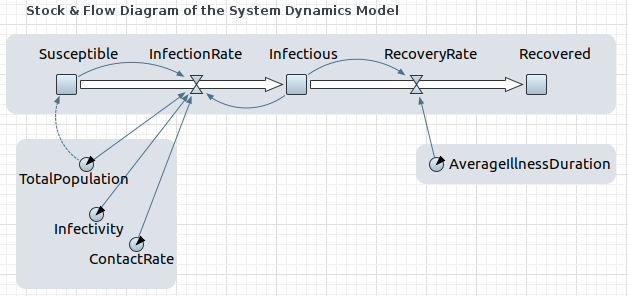
\includegraphics[width=.5\textwidth, angle=0]{./fig/SIR_SD_STOCKFLOW_DIAGRAMM.png}
	\caption{Visual System Dynamics Diagram of the SIR model in AnyLogic Personal Learning Edition 8.3.1.}
	\label{fig:sir_stockflow_diagram}
\end{figure}

Still, implementing System Dynamics directly in code is not as straight forward and involves numerical integration which can be quite tricky to get right. Thus, the aim of this paper is to look into how System Dynamics models can be implemented in code correctly without the use of a simulation package. We use the well known SIR model \cite{kermack_contribution_1927} from epidemiology to demonstrate our approach.

Our language of choice is Haskell because it emphasises a declarative programming style in which one describes \textit{what} instead of \textit{how} to compute. Further it allows to rule out interference with non-deterministic influences or side-effects already at compile-time. This is of fundamental importance for System Dynamics because it behaves completely deterministic and involves no stochastics or non-determinism whatsoever. Also, we make use of Functional Reactive Programming which allows to express continuous-time systems in a functional way. 

We show that by this approach we can arrive at correct-by-construction implementations of System Dynamic models. This means that the correctness of the code is obvious because we have closed the gap between the model specification and its implementation. Thus, the contribution of the paper is the demonstration of how to implement correct-by-construction System Dynamics simulations using Haskell and Functional Reactive Programming.
\chapter{Agents}

TODO: general agents: what they are and what they are not


\section{Agent Models}
Agent Models are NOT specific to any programming language implementation but should in theory be implementable in all languages which support the required primitives of the model or which allows the primitives of the model to be mapped to primitives of the language. Of course this says nothing about how well a language is suited to implement a given agent model and how readable and natural the mapping and implementation is. \\

Start from wooldridge 2.6 (look at the original papers which inspired the 2.6 chapter) and weiss book and the original papers those chapter is based upon. Look into denotational semantics of actor model. Look also in functional models of czesar ionescu. why: this is the major contribution of my thesis and is new knowledge. Must find intuitive, original and creative approach. \\
From functional agent models (e.g. Wooldridge) to implementation of ACE in Haskell (this should go into research-proposal introduction)

\subsection{Actors}

\subsection{TODO: is FRP an agent-model?}
It is specific to (pure) functional programming languages and can only be implemented with very cumbersome overhead in object-oriented languages like Java.
So maybe we can do that in Scala and LISP as well?

\section{Implementing Agents}
In the end it all boils down to 1. the agent-model and 2. how the agent-model is implemented in the according language. Of course both points influence each other: functional languages will come up with a different agent-model (e.g. hybrid like yampa) than object-oriented ones (e.g. actors).

The only constants are: see actors
%*******************************************************************************
%*********************************** Agent-based computational Economics *****************************
%*******************************************************************************

\chapter{ACE} 
read ACE introduction papers, summarize in this research-proposal

look into computable economics book: \url{http://www.e-elgar.com/shop/computable-economics}

TODO: the reading should pull out the essence of what types of ACE there are and what features each type has (continuous/discrete time, complex agent communication, equilibriua, networks amongst agents,...)

NOTE: I REALLY need to work out what is special in ACE? what is the unique property of ACE AS compared to other ABM/S? Conjecture: equilibrium of dynamics is the central aspect.
\url{http://www2.econ.iastate.edu/tesfatsi/ace.htm}

\cite{mandel_2015} Agent-based modeling and economic theory: where do we stand? - Ballot, Mandel, Vignes \\
\cite{richiardi_2007} Agent-based Computational Economics. A Short Introduction - Richiardi \\
\cite{tesfatsion_2006} Agent-based computational economics: a constructive approach to economic theory - tesfatsion \\
\cite{kleinberg_easley_2015} Introduction to computer science and economic theory - blume, easley, kleinberg \\
\cite{tesfatsion_2002} agent-based computational economics - tesfatsion 



The book \cite{KirmanComplex2010} is a critique of classic economics with the triple of rational agents, "average" inidividuum, equilibrium theory. Although it does not mention ACE it  can be seen as an important introduction to the approach of ACE as it introduces many important concepts and views dominant in ACE. Also ACE can be seen as an approach of tackling the problems introduced in this book: \\

page 6: "the view of economy is much closer to that of social insects than to the traditional view of how economies function." \\
page 7: "... main argument that it is the interaction between individuals that is at the heart of the explanation of many macroeconomic phenomena..." \\
page 15: "problem of equilibrium is information" \\
page 21: "the theme of this book will be that the very fact individuals interact with each other causes aggregate behaviour to be different from that of individuals" \\


\section{TODO: market-models}
find all agent-based market models (gintis, gode and sunder,...), read gintis equilibrium stuff and summarize in the paper: EDSL for agent-based market-simulations

\section{Related Research}

TODO: \cite{Kirman2001}
TODO: \cite{Kaminski2013}
TODO: how economists can get a life  tesfatsion

\section{Agent Models in ACE}
"[...] computational modelling of economic processes (including whole economies) as open-ended dynamic systems of interacting agents." Leigh Tesfatsion

TODO: look into the models of agents dominant in ACE. They seem to be more of reactive, continuous nature

depending on the model ACE \\

properties
\begin{itemize}
\item Discrete entities with own goals and behaviour
\item Not necessarily own thread of control
\item Capable to adapt 
\item Capable to modify their behaviour
\item Proactive behaviour: actions depending on motivations generated from their internal state
\end{itemize}

same as in classic ABMs: decentralised: there is no place where global system behaviour (system dynamics) is defined. Instead individual agents interact with each other and their environment to produce complex collective behaviour patterns.

also central to ACE: emergent properties. They show up in the form of equilibria

spatial / geo-spatial aspects not as dominant as in other fields of ABMs. TODO: is this really true?
more important: networks between agents

what are goals in ACE?
what are behaviour in ACE?

behaviour and intelligence is not the main focus

they can be seen as a continuous transformation process

% Part II: Practical Approach
%*******************************************************************************
%*********************************** Agent-based computational Economics *****************************
%*******************************************************************************

\chapter{Haskell} 
NOTE: this chapter should be the very first implementation chapter as the approach of Haskell lays the very foundations for the functional approach by introducing the basic functional concepts

So far the literature on agent-based modelling \& simulation (ABM/S) hasn't focused much on models for functional agents and is lacking a proper treatment of implementing agents in pure-functional languages like Haskell. This paper looks into how agents can be specified functionally and then be implemented properly in the pure functional language Haskell. The functional agent-model is inspired by wooldridge 2.6. The programming paradigm used to implement the agents in Haskell is functional reactive programming (FRP) where the Yampa framework will be used. The paper will show that specifying and implementing agents in a pure functional language like Haskell has many advantages over classical object-oriented, concurrent ones but needs also more careful considerations to work properly.
\end{abstract}

TODO: read \cite{backus_can_1978}

The state-of-the-art approach to implementing Agents are object-oriented methods and programming as the metaphor of an Agent as presented above lends itself very naturally to object-orientation (OO). The author of this thesis claims that OO in the hands of inexperienced or ignorant programmers is dangerous, leading to bugs and hardly maintainable and extensible code. The reason for this is that OO provides very powerful techniques of organising and structuring programs through Classes, Type Hierarchies and Objects, which, when misused, lead to the above mentioned problems. Also major problems, which experts face as well as beginners are 1. state is highly scattered across the program which disguises the flow of data in complex simulations and 2. objects don’t compose as well as functions. The reason for this is that objects always carry around some internal state which makes it obviously much more complicated as complex dependencies can be introduced according to the internal state.
All this is tackled by (pure) functional programming which abandons the concept of global state, Objects and Classes and makes data-flow explicit. This then allows to reason about correctness, termination and other properties of the program e.g. if a given function exhibits side-effects or not. Other benefits are fewer lines of code, easier maintainability and ultimately fewer bugs thus making functional programming the ideal choice for scientific computing and simulation and thus also for ACE. A very powerful feature of functional programming is Lazy evaluation. It allows to describe infinite data-structures and functions producing an infinite stream of output but which are only computed as currently needed. Thus the decision of how many is decoupled from how to (Hughes, J. (1989). Why functional programming matters. Comput. J., 32(2):98–107.).
The most powerful aspect using pure functional programming however is that it allows the design of embedded domain specific languages (EDSL). In this case one develops and programs primitives e.g. types and functions in a host language (embed) in a way that they can be combined. The combination of these primitives then looks like a language specific to a given domain, in the case of this thesis ACE. The ease of development of EDSLs in pure functional programming is also a proof of the superior extensibility and composability of pure functional languages over OO (Henderson P. (1982). Functional Geometry. Proceedings of the 1982 ACM Symposium on LISP and Functional Programming.).
One of the most compelling example to utilize pure functional programming is the reporting of Hudak (Hudak P., Jones M. (1994). Haskell vs. Ada vs. C++ vs. Awk vs. ... An Experiment in Software Prototyping Productivity. Department of Computer Science, Yale University.)  where in a prototyping contest of DARPA the Haskell prototype was by far the shortest with 85 lines of code. Also the Jury mistook the code as specification because the prototype did actually implement a small EDSL which is a perfect proof how close EDSL can get to and look like a specification.

Functional languages can best be characterized by their way computation works: instead of \textit{how} something is computed, \textit{what} is computed is described. Thus functional programming follows a declarative instead of an imperative style of programming. The key points are:
\begin{itemize}
\item No assignment statements - variables values can never change once given a value.
\item Function calls have no side-effect and will only compute the results - this makes order of execution irrelevant, as due to the lack of side-effects the logical point in \textit{time} when the function is calculated within the program-execution does not matter.
\item higher-order functions
\item lazy evaluation
\item Looping is achieved using recursion, mostly through the use of the general fold or the more specific map.
\item Pattern-matching
\end{itemize}


\section{Related Research}
NOTE: has been moved to functional agents paper

\section{Structuring pure functional programs}
Of course the basic pure functional primitives alone do not make a well structured functional program by themselves as the usage of classes, interfaces, objects and inheritance alone does not make a well structured object-oriented program. What is needed are \textit{patterns} how to use the primitives available in pure functional programs to arrive at well structure programs. In object-orientation much work has been done in the 90s by the highly influential book \cite{gamma_design_1994} whereas in functional programming the major inventions were also done in the 90s by the invention of Monads through \cite{Moggi1989}, \cite{Wadler1990} and \cite{Wadler1995} and beginning of the 2000s by the invention of Arrows through \cite{Hughes2000}.

\subsection{Higher Order Functions \& Monads}
map \& fmap, foldl, applicatives
\cite{hutton_programming_2007} gives a great overview and motivation for using fmap, applicatives and Monads. TODO: explain Monads

\subsection{Arrows}
\cite{Hughes2004} is a great tutorial about \textit{Arrows} which are very well suited for structuring functional programs with effects.

\begin{quote}
Just like monads, arrow types are useful for the additional operations they support, over and above those that every arrow provides.
\end{quote}

The main difference between Monads and Arrows are that where monadic computations are parameterized only over their output-type, Arrows computations are parameterised both over their input- and output-type thus making Arrows more general.

\begin{quote}
In real applications an arrow often represents some kind of a process, with an input channel of type a, and an output channel of type b.
\end{quote}

In the work \cite{Hughes2004} an example for the usage for Arrows is given in the field of circuit simulation. They use previously introduced streams to advance the simulation in discrete steps to calculate values of circuits thus the implementation is a form of \textit{discrete event simulation} - which is in the direction we are heading already with ABM/S. Also the paper mentions Yampa which is introduced in the section (TODO: reference) on functional reactive programming.

\section{Frameworks}

\subsection{Functional reactive programming (FRP)}
FRP is a paradigm for programming hybrid systems which combine continuous and discrete components. Time is explicitly modelled: there is a continuous and synchronous time flow.  \\

there have been many attempts to implement FRP in frameworks which each has its own pro and contra. all started with fran, a domain specific language for graphics and animation and at yale FAL, Frob, Fvision and Fruit were developed. The ideas of them all have then culminated in Yampa which is the reason why it was chosen as the FRP framework. Also, compared to other frameworks it does not distinguish between discrete and synchronous time but leaves that to the user of the framework how the time flow should be sampled (e.g. if the sampling is discrete or continuous - of course sampling always happens at discrete times but when we speak about discrete sampling we mean that time advances in natural numbers: 1,2,3,4,... and when speaking of continuous sampling then time advances in fractions of the natural numbers where the difference between each step is a real number in the range of [0..1]) \\

time- and space-leak: when a time-dependent computation falls behind the current time. TODO: give reason why and how this is solved through Yampa. \\
Yampa solves this by not allowing signals as first-class values but only allowing signal functions which are signal transformers which can be viewed as a function that maps signals to signals. A signal function is of type SF which is abstract, thus it is not possible to build arbitrary signal functions. Yampa provides primitive signal functions to define more complex ones and utilizes arrows \cite{Hughes2004} to structure them where Yampa itself is built upon the arrows: SF is an instance of the Arrow class. \\

Fran, Frob and FAL made a significant distinction between continuous values and discrete signals. Yampas distinction between them is not as great. Yampas signal-functions can return an Event which makes them then to a signal-stream - the event is then similar to the Maybe type of Haskell: if the event does not signal then it is NoEvent but if it Signals it is Event with the given data. Thus the signal function always outputs something and thus care must be taken that the frequency of events should not exceed the sampling rate of the system (sampling the continuous time-flow). TODO: why? what happens if events occur more often than the sampling interval? will they disappear or will the show up every time? \\

switches allow to change behaviour of signal functions when an event occurs. there are multiple types of switches: immediate or delayed, once-only and recurring - all of them can be combined thus making 4 types. It is important to note that time starts with 0 and does not continue the global time when a switch occurs. TODO: why was this decided? \\

\cite{Nilsson2002} give a good overview of Yampa and FRP. Quote: "The essential abstraction that our system captures is time flow". Two \textit{semantic} domains for progress of time: continuous and discrete. \\

The first implementations of FRP (Fran) implemented FRP with synchronized stream processors which was also followed by \cite{Wan2000}. Yampa is but using continuations inspired by Fudgets. In the stream processors approach "signals are represented as time-stamped streams, and signal functions are just functions from streams to streams", where "the Stream type can be implemented directly as (lazy) list in Haskell...":
\begin{lstlisting}[frame=single]
type Time = Double
type SP a b = Stream a -> Stream b
newtype SF a b = SF (SP (Time, a) b)
\end{lstlisting}
Continuations on the other hand allow to freeze program-state e.g. through closures and partial applications in functions which can be continued later. This requires an indirection in the Signal-Functions which is introduced in Yampa in the following manner. 
\begin{lstlisting}[frame=single]
type DTime = Double

data SF a b = 
	SF { sfTF :: DTime -> a -> (SF a b, b)
\end{lstlisting}
The implementer of Yampa call a signal function in this implementation a \textit{transition function}. It takes the amount of time which has passed since the previous time step and the durrent input signal (a). It returns a \textit{continuation} of type SF a b determining the behaviour of the signal function on the next step (note that exactly this is the place where how one can introduce stateful functions like integral: one just returns a new function which encloses inputs from the previous time-step) and an \textit{output sample} of the current time-step. \\

When visualizing a simulation one has in fact two flows of time: the one of the user-interface which always follows real-time flow, and the one of the simulation which could be sped up or slowed down. Thus it is important to note that if I/O of the user-interface (rendering, user-input) occurs within the simulations time-frame then the user-interfaces real-time flow becomes the limiting factor. Yampa provides the function embedSync which allows to embed a signal function within another one which is then run at a given ratio of the outer SF. This allows to give the simulation its own time-flow which is independent of the user-interface. \\

One may be initially want to reject Yampa as being suitable for ABM/S because one is tempted to believe that due to its focus on continuous, time-changing signals, Yampa is only suitable for physical simulations modelled explicitly using mathematical formulas (integrals, differential equations,...) but that is not the case. Yampa has been used in multiple agent-based applications: \cite{Hudak2003} uses Yampa for implementing a robot-simulation, \cite{Courtney2003} implement the classical Space Invaders game using Yampa, the thesis of \cite{Meisinger2010} shows how Yampa can be used for implementing a Game-Engine, \cite{Frag2005} implemented a 3D first-person shooter game with the style of Quake 3 in Yampa. Note that although all these applications don't focus explicitly on agents and agent-based modelling / simulation all of them inherently deal with kinds of agents which share properties of classical agents: game-entities, robots,... Other fields in which Yampa was successfully used were programming of synthesizers (TODO: cite), Network Routers, Computer Music Development and various other computer-games. This leads to the conclusion that Yampa is mature, stable and suitable to be used in functional ABM/S. \\
Jason Gregory (Game Engine Architecture) defines Computer-Games as "soft real-time interactive agent-based computer simulations".

To conclude: when programming systems in Haskell and Yampa one describes the system in terms of signal functions in a declarative manner (functional programming) using the EDSL of Yampa. During execution the top level signal functions will then be evaluated and return new signal functions (transition functions) which act as continuations: "every signal function in the dataflow graph returns a new continuation at every time step".

"A major design goal for FRP is to free the programmer from 'presentation' details by providing the ability to think in terms of 'modeling'. It is common that an FRP program is concise enough to also serve as a specification for the problem it solves" \cite{Wan2000}. This quotation describes exactly one of the strengths using FRP in ACE \\

\section{Reasoning}
Give example by showing reasoning in ACE: convergence, correctness,...
Look into Graham Huttons Book on Haskell: there are suggestions for further reading

\subsection{Time and Semantics}
\cite{Wan2000} discuss the semantic framework of FRP. Very difficult to understand and full of corollaries and theorems and proofs, have to study in depth at another time.

\section{Determinism}
no concurrent execution: deterministic \\

deterministic: can use random-numbers but to be reproducible/deterministic one has to specify the same seed or even provide an own RNG-implementation (which is easily possible using the RNG in haskell) \\

it is of most importance in simulations to be reproducible under given conditions: two runs with the same input (e.g. time, agent-count, parameters, RNG seeds) should result in the exact same results otherwise the simulation-software is of very little benefit.

\subsection{EDSL}
In this paper I present an EDSL which allows to formulate models for agent-based market-simulations which can be directly run in a Haskell framework implemented for this. Thus the distinction between model specification and programming vanishes - the model specification becomes the actual code. The major novelty of this EDSL is that it allows to model the system in a qualitative way: relations among formulas are expressed which can be understood as a kind of non-causal modelling. TODO: better understand what qualitative modelling/simulation in ACE is.

\cite{Henderson1982} gives a wonderful way of constructing an EDSL do denotationally construct an Escher-Picture.

\section{Implementations}
idea: can we implement a message between two agents through events? thus two states: waiting for messages, processing messages. BUT: then sending a message \textit{will take some time}

NOTE: it is important to make a difference about whether the simulation will dynamically \textit{add} or \textit{remove} agents during execution. If this is not the case, a simple par-switch is possible to run ALL agent SF in parallel. If dynamically changes to the agent-population should be part of the simulation, then the dpSwitch or dpSwitchB should be used. Also it should be possible to start/stop agents: if they are inactive then they should have no running SF because would use up resources. Inactive means: doing nothing, also not awaiting something/"doing nothing in the sense that DOING something which is nothing - the best criteria to decide if an agent can be set inactive is when the event which decides if the agents SF should be started comes from outside e.g. if the agent is just statically "living" but not changing and then another agent will "ignite" the "living" agent then this is a clear criterion for being static without a running SF. \\

NOTE: the route-function will be used to distribute "messages" to the agents when they are communicating with each other \\

NOTE: \cite{Meisinger2010} argues that in Game-Engines (it is paraphrased in english, as the thesis was written in german): "communication among Game-Objects is always computer-game specific and must be implemented always new but the functionality of Game-objects can be built by combining independent functions and signal-functions which are fully reuse-able". Game-Objects can be understood as agents thus maybe this also holds true for agent-based simulation. \cite{Meisinger2010} thus distinguishes between normal functions e.g. mathematical functions, signal functions which depend on output since its creation in localtime and game-object functions which output depends on inputs AND time (which is but another input). \\

TODO: need a mechanism to address agents: if agent A wants to send a message to agent B and agent B wants to react by answering with a message to agent A then they must have a mechanism to address each other \\

TODO: design general input/output data-structures \\

TODO: design general agent SF \\

TODO: don't loose STM out of sight!

Wormholes in FRP? \\


\subsection{Testing}
TODO: look into \cite{Claessen2000}

\section{Performance}

\subsection{Active vs inactive Agents}
signalfunctions add up, multiple chains of events add up, need to remove inactive agents or exclude them somehow from computation chain: use freezing? \\

\subsection{Parallelism and Concurrency}

\cite{Bezirgiannis2013} puts special emphasis on concurrency and parallelism in implementing simulation framework in Haskell. TODO: explain deeper \\

Due to the pure-functional property of a agents SF (which fully describes the agents behaviour over time) all signal-functions of all agents should be able to run in parallel in each iteration as they are pure functional: they don't touch global/shared state. Also the routing and switching functions could be sped up using par. But Question: how is this possible in Yampa? \\

Wormholes in FRP? \\

%*******************************************************************************
%*********************************** Agent-based computational Economics *****************************
%*******************************************************************************

\chapter{Scala \& Actors} 
The Actor-Model, a model of concurrency, has been around since the paper \cite{Hewitt_1973} in 1973. It was a major influence in designing the concept of Agents and although there are important differences between Actors and Agents there are huge similarities thus the idea to use actors to build agent-based simulations comes quite natural. Although there are papers around using the actor model as basis for their ABMS unfortunately no proper theoretical treatment of using the actor-model in implementing agent-based simulations has been done so far. This paper looks into how the more theoretical foundations of the suitability of actor-model to ABMS and what the upsides and downsides of using it are.

\url{http://www.grids.ac.uk/Complex/ABMS/}

\cite{Bezirgiannis2013} describes in chapter 3.3 a naive clone of NetLogo in the Erlang programming language where each agent was represented as an Erlang process. The author claims the 1:1 mapping between agent and process to "be inherently wrong" because when recursively sending messages (e.g. A to B to A) it will deadlock as A is already awaiting Bs answer. Of course this is one of the problems when adopting Erlang/Scala with Akka/the Actor Model for implementing agents \textit{but it is inherently short-sighted to discharge the actor-model approach just because recursive messaging leads to a deadlock}. It is not a problem of the actor-model but merely a very problem with the communication protocol which needs to be more sophisticated than \cite{Bezirgiannis2013} described. The hypothesis is that the communication protocol will be in fact \textit{very highly application-specific} thus leading to non-reusable agents (across domains, they should but be re-usable within domains e.g. market-simulations) as they only understand the domain-specific protocol. This is definitely NOT a drawback but can't be solved otherwise as in the end (the content of the) communication can be understand to be the very domain of the simulation and is thus not generalizable. Of course specific patterns will show up like "multi-step handshakes" but they are again then specifically applied to the concrete domain.

\subsection{The Actor Model}
Read in the following order


\begin{enumerate}
\item \cite{Hewitt_1973}
\item \cite{Greif_1975}
\item \cite{Clinger_1981}
\item \cite{Agha_1986}
\item \cite{Agha_1997}
\item \cite{Hewitt_2007}
\item \cite{Hewitt_2010}
\item \cite{Agha_2004}
\end{enumerate}

upside: extreme huge number of agnts possible due to distributed and parallel technology 
downside: depends on system \& hardware: scheduler, system time, systime resolution (not very nice for scientific computation), much more complicated, debugging difficult due to concurrency, no global notion of time appart from systemtime, thus always runs in real-time, but there is no global notion of time in the actor model anyway, no EDSL full of technical details, no determinism, no reasoning

\subsection{Agents vs. Actors}
Agents more a high-level concept, Actors low level, technical concurrency primitives

\subsection{Actors are pure functional!}

\subsection{Hypothesis}
This makes simulations very difficult and also due to concurrency implementing a sync conversation among agents is very cumbersome. I have already experience with the Actor Model when implementing a small version of my Master-Thesis Simulation in Erlang which uses the Actor Model as well. For a continuous simulation it was actually not that bad but the problem there was that between a round-trip between 2 agents other messages could have already interfered - this was a problem when agents trade with each other, so one has to implement synchronized trading where only messages from the current agent one trades with are allowed otherwise budget constraints could be violated. Thus I think Erlang/Akka/Actor Model is better suited for distributed high-tolerance concurrent/parallel systems instead for simulations. Note: this is definitely a major point I have to argue in my thesis: why I am rejecting the actor model.

AKKA: thus my prediction is: akka/actor model is very well suited to simulations which 1. dont rely on global time 2. dont have multi-step conversations: interactions among agents which are only question-answer. TODO: find some classical simulation model which satisfies these criterias.

\section{Actor Model implementations}
It is important to note that the actor-model is not tied to any particular programming language and could be (and is) implemented in different types of languages like Java (Object-Oriented), Haskell (pure functional) and Scala (mix of functional and Object-Oriented).

\subsection{Erlang}
TODO: erlang is an old implementation of the actor model

\subsection{Akka}
TODO: akka is a modern implementation of the actor model

\subsection{Haskell}
TODO: can implement actor-model using forkIO and STM


\section{Theoretical reflections}

\subsection{The problem of time}
 how can we simulate global time? how can we implement multistep conversations (by futures)?

The real problem seems to be concurrency but i feel we can simulate concurrency by synchronizing to continuous time. computations are carried out after another but because time is explicitly modelled they happen logically at the same time. these rules hold: an agent cannot be in two conversations at the same time, the agent can be in only one or none conversation at a given time t.

What if time is of no importance and only the continuous dynamics are of interest?

To put it another way: real concurrency (with threads) makes time implicit which is what one does NOT want in simulation. Maybe FRP is the way to go because it allows to explicitly model continuous and discrete time, but I have to get into FRP first to make a proper judgement about its suitability.

\subsection{Conversations}
new concept: not single, async messages, but syncronous conversations which (can) take time = multiple synchronous messages between agents which (can) change the state of an agent in the end.

\section{Example implementation}

\subsection{Wildfire with/without wind}
"This is a model of a wildfire. Vegetation is modeled as grid cells - agents in discrete space. The burning time of a cell is proportional to the amount of “fuel” in the cell, which is randomly generated at the model startup. While burning, the cell may cause ignition in adjacent cells. You can cause the initial ignition by clicking a cell. The ignition may also be caused by a bomb dropped by the aircraft - an agent moving in continuous 2D space that overlaps the discrete space. This model, among other things, shows how the two types of space can be linked. The model is computationally very efficient because there are no time steps in this model; the behavior of vegetation cells and the aircraft is defined in the form of a statechart. Unlike in the full version, in this model wind is not taken into consideration."

"This is a model of a wildfire. Vegetation is modeled as grid cells - agents in discrete space. The burning time of a cell is proportional to the amount of “fuel” in the cell, which is randomly generated at the model startup. While burning, the cell may cause ignition in adjacent cells. The probability of ignition depends on the wind direction (which you can change on the fly). You can cause the initial ignition by clicking a cell. The ignition may also be caused by a bomb dropped by the aircraft – an agent moving in continuous 2D space that overlaps the discrete space. This model, among other things, shows how the two types of space can be linked. The model is computationally very efficient because there are no time steps in this model; the behavior of vegetation cells and the aircraft is defined in the form of a statechart."

\begin{enumerate}
\item No time steps.
\item One-Step interaction.
\end{enumerate}

\subsection{Discrete SIR/S}
\begin{enumerate}
\item Discrete time steps.
\item One-Step interaction.
\end{enumerate}

\section{Decentralized bartering}

\begin{enumerate}
\item Continuous time.
\item Multi-Step interactions.
\end{enumerate}

\section{Further Research}
\subsection{Pure functional approach}
\subsection{Explicit time}

\section{Conclusion}
\subsection{Real concurrency not needed in simulation}
AKKA is nice but I think the actor model is not very well suited for simulations  due to inherent concurrency where time is implicit. 

real concurrency is not needed: simultaneous events can be modeled through explicit time but calculated sequential - when we reduce agents to process only one message after another and not multiple concurrently. thus true parallelism is only a technical detail for performance enhancement.

%*******************************************************************************
%*********************************** Agent-based computational Economics *****************************
%*******************************************************************************

\chapter{Lisp} 
Why LISP: the oldest language and functional. Has extremely powerful properties: homoiconic: data = code = data. We ask how those can be utilized to implement agent-based simulations in economics.

NEPI^2 framework
%*******************************************************************************
%*********************************** Agent-based computational Economics *****************************
%*******************************************************************************

\chapter{Java \& Repast} 
Is a state-of-the-art OO method. This is the golden standard to be compared to the other functional approaches to show where the differences are and what the up- and downs are.

These tools are state-of-the-art in ABM/S and ACE and are included to show how one can perform scenarios (see below) with these tools.
Java is the state-of-the-art programming language in ABM/S and ACE and is thus included as well as a benchmark against such a state-of-the-art.


% Part III: Reflections

% Part IV: ?

% ********************************** Back Matter *******************************
% Backmatter should be commented out, if you are using appendices after References
%\backmatter

% ********************************** Bibliography ******************************
\begin{spacing}{0.9}

% To use the conventional natbib style referencing
% Bibliography style previews: http://nodonn.tipido.net/bibstyle.php
% Reference styles: http://sites.stat.psu.edu/~surajit/present/bib.htm

\bibliographystyle{apalike}
%\bibliographystyle{unsrt} % Use for unsorted references  
%\bibliographystyle{plainnat} % use this to have URLs listed in References
\cleardoublepage
\bibliography{References/references} % Path to your References.bib file


% If you would like to use BibLaTeX for your references, pass `custombib' as
% an option in the document class. The location of 'reference.bib' should be
% specified in the preamble.tex file in the custombib section.
% Comment out the lines related to natbib above and uncomment the following line.

%\printbibliography[heading=bibintoc, title={References}]


\end{spacing}

% ********************************** Appendices ********************************

% \begin{appendices} % Using appendices environment for more functunality
% % ******************************* Thesis Appendix A ****************************
\chapter{How to install \LaTeX} 

\section*{Windows OS}

\subsection*{TeXLive package - full version}
\begin{enumerate}
\item	Download the TeXLive ISO (2.2GB) from\\
\href{https://www.tug.org/texlive/}{https://www.tug.org/texlive/}
\item	Download WinCDEmu (if you don't have a virtual drive) from \\
\href{http://wincdemu.sysprogs.org/download/}
{http://wincdemu.sysprogs.org/download/}
\item	To install Windows CD Emulator follow the instructions at\\
\href{http://wincdemu.sysprogs.org/tutorials/install/}
{http://wincdemu.sysprogs.org/tutorials/install/}
\item	Right click the iso and mount it using the WinCDEmu as shown in \\
\href{http://wincdemu.sysprogs.org/tutorials/mount/}{
http://wincdemu.sysprogs.org/tutorials/mount/}
\item	Open your virtual drive and run setup.pl
\end{enumerate}

or

\subsection*{Basic MikTeX - \TeX~ distribution}
\begin{enumerate}
\item	Download Basic-MiK\TeX (32bit or 64bit) from\\
\href{http://miktex.org/download}{http://miktex.org/download}
\item	Run the installer 
\item	To add a new package go to Start >> All Programs >> MikTex >> Maintenance (Admin) and choose Package Manager
\item	Select or search for packages to install
\end{enumerate}

\subsection*{TexStudio - \TeX~ editor}
\begin{enumerate}
\item	Download TexStudio from\\
\href{http://texstudio.sourceforge.net/\#downloads}
{http://texstudio.sourceforge.net/\#downloads} 
\item	Run the installer
\end{enumerate}

\section*{Mac OS X}
\subsection*{MacTeX - \TeX~ distribution}
\begin{enumerate}
\item	Download the file from\\
\href{https://www.tug.org/mactex/}{https://www.tug.org/mactex/}
\item	Extract and double click to run the installer. It does the entire configuration, sit back and relax.
\end{enumerate}

\subsection*{TexStudio - \TeX~ editor}
\begin{enumerate}
\item	Download TexStudio from\\
\href{http://texstudio.sourceforge.net/\#downloads}
{http://texstudio.sourceforge.net/\#downloads} 
\item	Extract and Start
\end{enumerate}


\section*{Unix/Linux}
\subsection*{TeXLive - \TeX~ distribution}
\subsubsection*{Getting the distribution:}
\begin{enumerate}
\item	TexLive can be downloaded from\\
\href{http://www.tug.org/texlive/acquire-netinstall.html}
{http://www.tug.org/texlive/acquire-netinstall.html}.
\item	TexLive is provided by most operating system you can use (rpm,apt-get or yum) to get TexLive distributions
\end{enumerate}

\subsubsection*{Installation}
\begin{enumerate}
\item	Mount the ISO file in the mnt directory
\begin{verbatim}
mount -t iso9660 -o ro,loop,noauto /your/texlive####.iso /mnt
\end{verbatim}

\item	Install wget on your OS (use rpm, apt-get or yum install)
\item	Run the installer script install-tl.
\begin{verbatim}
	cd /your/download/directory
	./install-tl
\end{verbatim}
\item	Enter command `i' for installation

\item	Post-Installation configuration:\\
\href{http://www.tug.org/texlive/doc/texlive-en/texlive-en.html\#x1-320003.4.1}
{http://www.tug.org/texlive/doc/texlive-en/texlive-en.html\#x1-320003.4.1} 
\item	Set the path for the directory of TexLive binaries in your .bashrc file
\end{enumerate}

\subsubsection*{For 32bit OS}
For Bourne-compatible shells such as bash, and using Intel x86 GNU/Linux and a default directory setup as an example, the file to edit might be \begin{verbatim}
edit $~/.bashrc file and add following lines
PATH=/usr/local/texlive/2011/bin/i386-linux:$PATH; 
export PATH 
MANPATH=/usr/local/texlive/2011/texmf/doc/man:$MANPATH;
export MANPATH 
INFOPATH=/usr/local/texlive/2011/texmf/doc/info:$INFOPATH;
export INFOPATH
\end{verbatim}
\subsubsection*{For 64bit OS}
\begin{verbatim}
edit $~/.bashrc file and add following lines
PATH=/usr/local/texlive/2011/bin/x86_64-linux:$PATH;
export PATH 
MANPATH=/usr/local/texlive/2011/texmf/doc/man:$MANPATH;
export MANPATH 
INFOPATH=/usr/local/texlive/2011/texmf/doc/info:$INFOPATH;
export INFOPATH

\end{verbatim}



%\subsection{Installing directly using Linux packages} 
\subsubsection*{Fedora/RedHat/CentOS:}
\begin{verbatim} 
sudo yum install texlive 
sudo yum install psutils 
\end{verbatim}


\subsubsection*{SUSE:}
\begin{verbatim}
sudo zypper install texlive
\end{verbatim}


\subsubsection*{Debian/Ubuntu:}
\begin{verbatim} 
sudo apt-get install texlive texlive-latex-extra 
sudo apt-get install psutils
\end{verbatim}

% % ******************************* Thesis Appendix B ********************************

\chapter{Installing the CUED class file}

\LaTeX.cls files can be accessed system-wide when they are placed in the
<texmf>/tex/latex directory, where <texmf> is the root directory of the user’s \TeX installation. On systems that have a local texmf tree (<texmflocal>), which
may be named ``texmf-local'' or ``localtexmf'', it may be advisable to install packages in <texmflocal>, rather than <texmf> as the contents of the former, unlike that of the latter, are preserved after the \LaTeX system is reinstalled and/or upgraded.

It is recommended that the user create a subdirectory <texmf>/tex/latex/CUED for all CUED related \LaTeX class and package files. On some \LaTeX systems, the directory look-up tables will need to be refreshed after making additions or deletions to the system files. For \TeX Live systems this is accomplished via executing ``texhash'' as root. MIK\TeX users can run ``initexmf -u'' to accomplish the same thing.

Users not willing or able to install the files system-wide can install them in their personal directories, but will then have to provide the path (full or relative) in addition to the filename when referring to them in \LaTeX.


% \end{appendices}

% *************************************** Index ********************************
\printthesisindex % If index is present

\end{document}
